\chapter{Die praktische Umsetzung des Angriffs}

Dieses Kapitel beschreibt die Implementierungen und Anwendungen, die im Zuge der Arbeit entstanden sind. Insbesondere wird auf die Programme eingegangen, mit denen die Machbarkeit des Angriffs praktisch verifiziert wurde. Zuerst wurde die Manipulation der Telefonnummer in einer verschlüsselten und kodierten Setup-Nachricht umgesetzt. Im Anschluss wurde der Angriff von der Identifikation des Opfers, über die Identifikation der Setup-Nachricht, bis hin zu deren Manipulation in einer Testumgebung mit virtualisierter Funkschnittstelle durchgeführt. Die Beschreibung der Einrichtung und Konfiguration der verwendeten Testumgebung ist im Anhang in \autoref{hdl:a_einrichtung_testumgebung} zu finden.

\section{Die Virtualisierung der physikalischen Schicht der Um-Schnittstelle}

Für die Verifikation des \ac{MitM}-Angriffs wurde die physikalische Schicht der \ac{Um}-Schnittstelle virtualisiert. Damit ist eine Kommunikation über das \ac{Um} möglich, ohne spezielle Transceiverhardware für \ac{MS}, \ac{BTS} und \ac{MitM} zu benötigen. Die Verwendung einer Testumgebung mit virtueller \ac{Um}-Schnittstelle hat mehrere Vorteile. Da für den Nachrichtenaustausch keine Transceiverhardware benötigt wird, kann deren Konfiguration und Implementierung als Fehlerquelle bei der Entwicklung ausgeschlossen werden. Datenflüsse können schnell und kostengünstig aufgezeichnet und analysiert werden, was bei der Softwareentwicklung die Überprüfung der Auswirkungen einer Änderung vereinfacht. Im Vergleich mit einer Testumgebung mit realer Funkschnittstelle kann die virtualisierte Testumgebung einfacher eingerichtet und konfiguriert werden. Zudem werden Probleme mit der Legalität einer \ac{BTS} und dem Funkverkehr auf für \ac{GSM} reservierten Frequenzbändern vermieden. 

Als Grundlage für die Implementierung kamen zwei mögliche Ansätze in Frage. Die in MATLAB\footnote{\url{https://de.mathworks.com}} geschriebene Virtualisierung der Funkschnittstelle von kkro\footnote{\url{https://github.com/kkroo/matphy}} und die angefangene Implementierung einer virtuellen \ac{BTS} im osmoBTS Projekt von Harald Welte\footnote{\url{https://github.com/osmocom/osmo-bts.git}}. Für die Masterarbeit wurde der zweite Ansatz verfolgt. Für die virtuelle \ac{BTS} fehlten zwar noch Teile der Funktionalität und das Gegenstück in osmocomBB, die Implementierung war aber deutlich aktueller. Des Weiteren konnte so die vorhandene Funktionalität aus osmocomBB, osmoBTS und der libosmocore Bibliothek genutzt werden.

Um die Übertragung auf der Funkschnittstelle nachzubilden, müssen Nachrichten die \ac{TDMA}/\ac{FDMA} Informationen der physikalischen Schicht des \ac{Um} enthalten (siehe \autoref{hdl:a_tdma_fdma}). Die \textbf{Frequenz} wird in \ac{GSM} über die \ac{ARFCN} festgelegt. Eine \ac{ARFCN} definiert eine Uplink- und eine Downlinkfrequenz, über die \ac{MS} und \ac{BTS} kommunizieren. Der \ac{TDMA}-Zeitschlitz legt den \textbf{physikalischen Kanal} der Nachricht fest, die \ac{FN} ihren \textbf{logischen Kanal} (siehe \autoref{hdl:logical-channels}). Durch physikalischen und logischen Kanal wird eindeutig festgelegt, wie die physikalische Schicht mit der Nachricht umgehen muss und über welchen \ac{SAP} sie diese an höhere Schichten weiterleitet. Auf dem \ac{Um} werden in der Regel auch Messungen der Signalqualität durchgeführt und übertragen. Für das virtuelle \ac{Um} sind diese weniger von Bedeutung, da alle Nachrichten mit gleicher Qualität übertragen werden.

Für die Virtualisierung sollen die Nachrichten des \ac{Um} statt über Funksignale zwischen Sockets auf einer Linux Maschine übertragen werden. Für die Kapselung von \ac{Um}"=Nach\-rich\-ten und deren Übertragung über \ac{UDP}/\ac{IP} bietet die libosmocore Bibliothek den \ac{GSMTAP}"=Header an. \ac{TAP} Header sind dazu gedacht, einem Analyse- oder Testgerät Informationen über den Datenverkehr einer Netzwerkschnittstelle zugänglich zu machen. Er übernimmt in Osmocom Projekten die Funktion des Wireshark-Dissektors bei der Aufzeichnung und Protokollierung des Nachrichtenverkehr auf dem \ac{Um} mit Wireshark. Von der \ac{IANA} wurde dem \ac{GSMTAP}-Dissektor der Port 4729 zugewiesen. \autoref{lst:gsmtap_hdr} zeigt den Aufbau des \ac{GSMTAP} Headers. \\

%\begin{adjustbox}{max width={0.95\textwidth}, padding=20pt 10pt 10pt 10pt, frame, center}
\begin{lstlisting}[caption={[Der Aufbau des GSMTAP-Headers]Der Aufbau des \ac{GSMTAP}-Headers, aus der libosmocore Bibliothek}, label={lst:gsmtap_hdr}, boxpos=c, frame=single, style=CStyle, numbers=none]
/*! \brief Structure of the GTMTAP pseudo-header */
struct gsmtap_hdr {
uint8_t version;	/*!< version, set to 0x01 currently */
uint8_t hdr_len;	/*!< length in number of 32bit words */
uint8_t type;		/*!< see GSMTAP_TYPE_* */
uint8_t timeslot;	/*!< timeslot (0..7 on Um) */

uint16_t arfcn;		/*!< ARFCN (frequency) */
int8_t signal_dbm;	/*!< signal level in dBm */
int8_t snr_db;		/*!< signal/noise ratio in dB */

uint32_t frame_number;	/*!< GSM Frame Number (FN) */

uint8_t sub_type;	/*!< Type of burst/channel, see above */
uint8_t antenna_nr;	/*!< Antenna Number */
uint8_t sub_slot;	/*!< sub-slot within timeslot */
uint8_t res;		/*!< reserved for future use (RFU) */
} __attribute__((packed));
\end{lstlisting}
%\end{adjustbox}

Die Implementierung des virtuellen \ac{Um} auf \ac{UDP}/\ac{IP} Basis verwendet den \ac{GSMTAP}"=Header für die Datenübertragung und erweitert damit seinen bisherigen Einsatzbereich. Das Feld \texttt{arfcn} enthält ein Uplink Flag und definiert so eindeutig die \textbf{Frequenz}. Der \textbf{physikalische Kanal} wird von \texttt{timeslot} definiert und der \textbf{logische Kanal} von \texttt{frame\_number} und \texttt{sub\_type}. Im Gegensatz zur Funkschnittstelle werden die Pakete auf dem virtuellen \ac{Um} dabei nicht in Bursts unterteilt. Es werden vollständige \ac{LAPDm}-Nachrichten von bis zu 184 Bit in einer \ac{GSMTAP}-Nachricht verpackt und über \ac{UDP}/\ac{IP} zur Gegenseite des virtuellen \ac{Um} geschickt. Durch die Verwendung des \ac{GSMTAP}-Headers erhält Wireshark außerdem out-of-the-box die Fähigkeit, den Datenverkehr auf dem virtuellen \ac{Um} darzustellen. Der \ac{GSMTAP}-Header ist nicht für die Übertragung von kanalkodierten und verschlüsselten Nachrichten konzipiert. Das virtuelle \ac{Um} unterstützt deshalb weder Kanalkodierung noch verschlüsselte Verbindungen. Für die praktische Durchführung des Angriffs wurde diese Funktionalität im osmoMITM Projekt implementiert (siehe \autoref{hdl:mitm_impl}).

Wegen der benötigten Broadcast Eigenschaften der Funkschnittstelle, eignen sich Linux Multicast-Sockets für die Kommunikation auf dem virtuellen \ac{Um}. Sie ermöglichen es einem \ac{BTS}-Prozess, Nachrichten an mehrere \ac{MS}-Prozesse zu versenden und umgekehrt. Für Multicast-Sockets ist auf Linux/Unix Systemen der \ac{IP}-Adressraum von 224.0.0 - 240.0.0.0 reserviert. Es gibt Multicast-Server-Sockets und Client-Sockets. Ein Server versendet Nachrichten an eine \ac{IP}-Adresse aus dem für Multicast reservierten Adressraum. Client-Sockets können diese empfangen, indem sie der Multicast Gruppe beitreten, die dieser \ac{IP}-Adresse entspricht. Die Konfiguration von Multicast kann dem Linux Benutzerhandbuch unter ip(7)\footnote{\url{http://man7.org/linux/man-pages/man7/ip.7.html}} entnommen werden. Um die Funkschnittstelle mit Multicast-Sockets zu simulieren, wird für Uplink und Downlink je ein Client und ein Server-Socket benötigt. \autoref{fig:virt-um-with-mcast} veranschaulicht die Verwendung der Multicast-Sockets im virtuellen \ac{Um}.

\begin{figure}[H]
	\centering 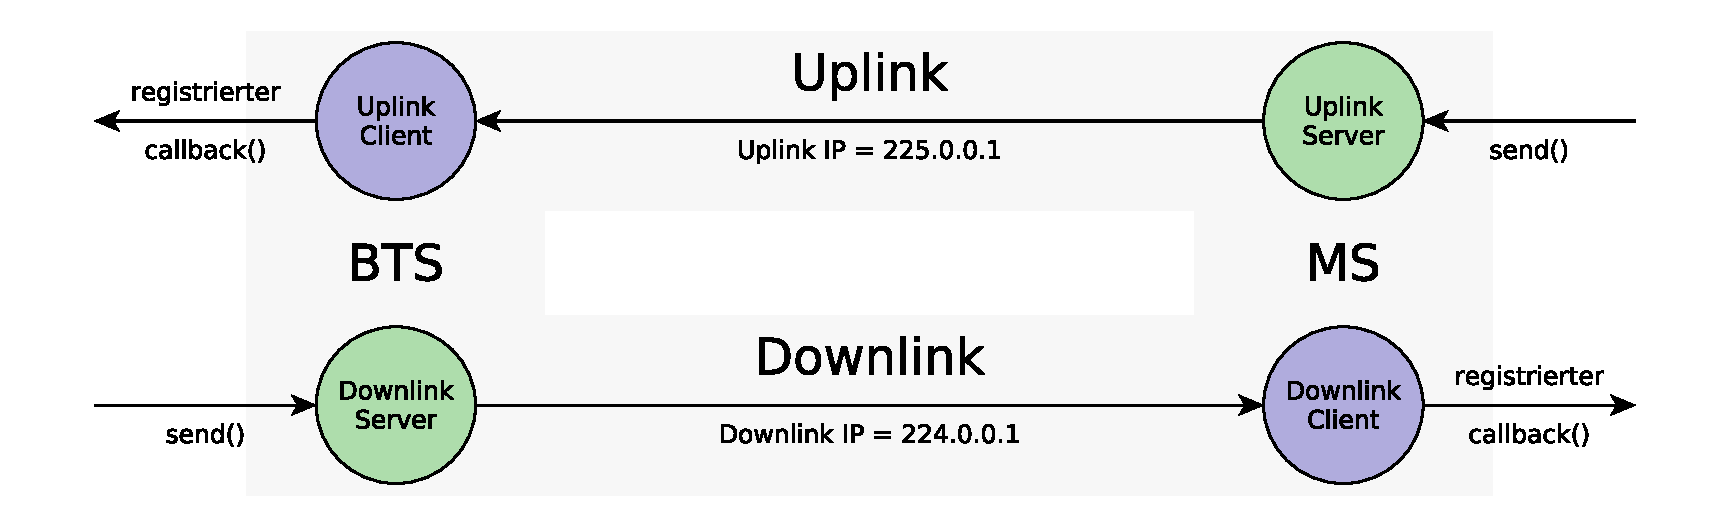
\includegraphics[width=0.9\textwidth]{figures/virt_um_with_multicast.pdf}
	\caption[Die Umsetzung der virtuellen Funkschnittstelle mit Multicast-Sockets]{Die Umsetzung der virtuellen Funkschnittstelle mit Multicast-Sockets, erstellt mit yEd} \label{fig:virt-um-with-mcast}
\end{figure}

Wie in \autoref{fig:virt-um-with-mcast} zu sehen, werden dabei je ein Server-Socket und ein Client-Socket zu Uplink und Downlink zusammengeschlossen. Die \ac{MS} kann über die \texttt{send()} Funktion Daten auf dem Uplink senden und über den \texttt{callback()} auf dem Downlink empfangen. Der Callback wird beim Start des virtuellen \ac{Um} registriert und ist die Methode, die vom Betriebssystem bei eingehenden Daten auf dem Socket aufgerufen wird. Umgekehrt dazu empfängt die \ac{BTS} auf dem Uplink und sendet auf dem Downlink. Durch die Realisierung mit Multicast-Sockets, können mehrere \ac{MS} und auch \ac{BTS} am virtuellen \ac{Um} angemeldet werden. Fügt man in \autoref{fig:virt-um-with-mcast} zum Beispiel eine weitere \ac{MS} hinzu und konfiguriert sie mit den selben \ac{IP}-Adressen für Uplink (225.0.0.1) und Downlink (224.0.0.1), werden alle vom \ac{BTS} gesendeten Nachrichten von beiden \ac{MS} empfangen. Für die Virtualisierung wurde in den beiden Osmocom Projekten osmocomBB und osmoBTS die Implementierung der physikalischen Schicht der Funkschnittstelle ersetzt. Da auf der Socket-Ebene die Anforderungen des virtuellen \ac{Um} auf \ac{MS} und \ac{BTS}-Seite die selben sind, wurde die damit zusammenhängende Funktionalität gekapselt. Die Datei \texttt{virt\_um.c} wird auf beiden Seiten als geteilte Ressource verwendet, automatisiert die Erstellung der Sockets, lässt sich mit Uplink und Downlink-Adressen sowie der \texttt{callback()} Methode konfigurieren und bietet die \texttt{send()} Funktion an.

Mit der Einbindung des virtuellen \ac{Um} in osmocomBB, osmoBTS und osmoMITM konnte der \ac{MitM}-Angriff erfolgreich simuliert und verifiziert werden. Auf der OsmoDevCon2017\footnote{\url{https://osmocom.org/projects/osmo-dev-con/wiki/OsmoDevCon2017}} wurde die Möglichkeit angesprochen, das virtuelle \ac{Um} in Zukunft in das Projekt osmoTester einzubinden. Da dadurch schnelle, hardwareunabhängige Tests möglich sind, kann es von Jenkins \footnote{\url{https://jenkins.io/}} zur Überprüfung korrekter Nachrichtenabläufe auf der Funkschnittstelle bei neuen Commits verwendet werden. Jenkins ist ein webbasiertes Tool für die Automatisierung des Software-Building Prozesses und wird dafür in Osmocom verwendet.

\section{OsmoBTS mit virtueller Um-Schnittstelle}

Das osmoBTS Projekt unterstützt unterschiedliche Hardware, was sich in der Ordnerstruktur widerspiegelt. So ist ein Großteil der \ac{BTS}-Funktionalität in einem Ordner \texttt{src/common}, der gemeinsam genutzte Funktionalität beinhaltet, ausgelagert. Er enthält vor allem die Implementierungen der hardwareunabhängigen, höheren Protokollschichten. Die Schnittstellen für die Unterstützung unterschiedlicher Transceiverhardware sind in mehreren weiteren Ordnern zu finden. Im Ordner \texttt{src/osmo-bts-trx} liegt zum Beispiel Code der Bursts auf einer \ac{UDP}-Schnittstelle von verschiedenen \ac{SDR}-Geräten entgegennimmt und verarbeitet. In \texttt{src/osmo-bts-sysmo} liegt eine Implementierung der physikalischen Schicht, mit der von sysmocom hergestellte \ac{BTS} Produkte über Ethernet angebunden werden können. Der Automake\footnote{\url{https://www.gnu.org/software/automake/manual}} Build-Prozess verbindet die Implementierungen der Protokollschichten und baut für jede der unterstützen Hardwaregeräte eine eigene Anwendung zusammen.

Für osmoBTS wurde in dieser Arbeit im Ordner \texttt{src/osmo-bts-virtual} die physikalische Schicht zur Unterstützung der virtuellen \ac{Um}-Schnittstelle implementiert. Sie erwartet und verarbeitet in \ac{GSMTAP} verpackte Nachrichten auf einem Multicast-Socket. Folgende Grafik zeigt die Schnittstellen der virtuellen \ac{BTS} (\texttt{osmo-bts-virt}) im Vergleich zu den anderen erwähnten \ac{BTS}-Anwendungen \texttt{osmo-bts-trx} und \texttt{osmo-bts-sysmo}.

\begin{figure}[H]
	\centering 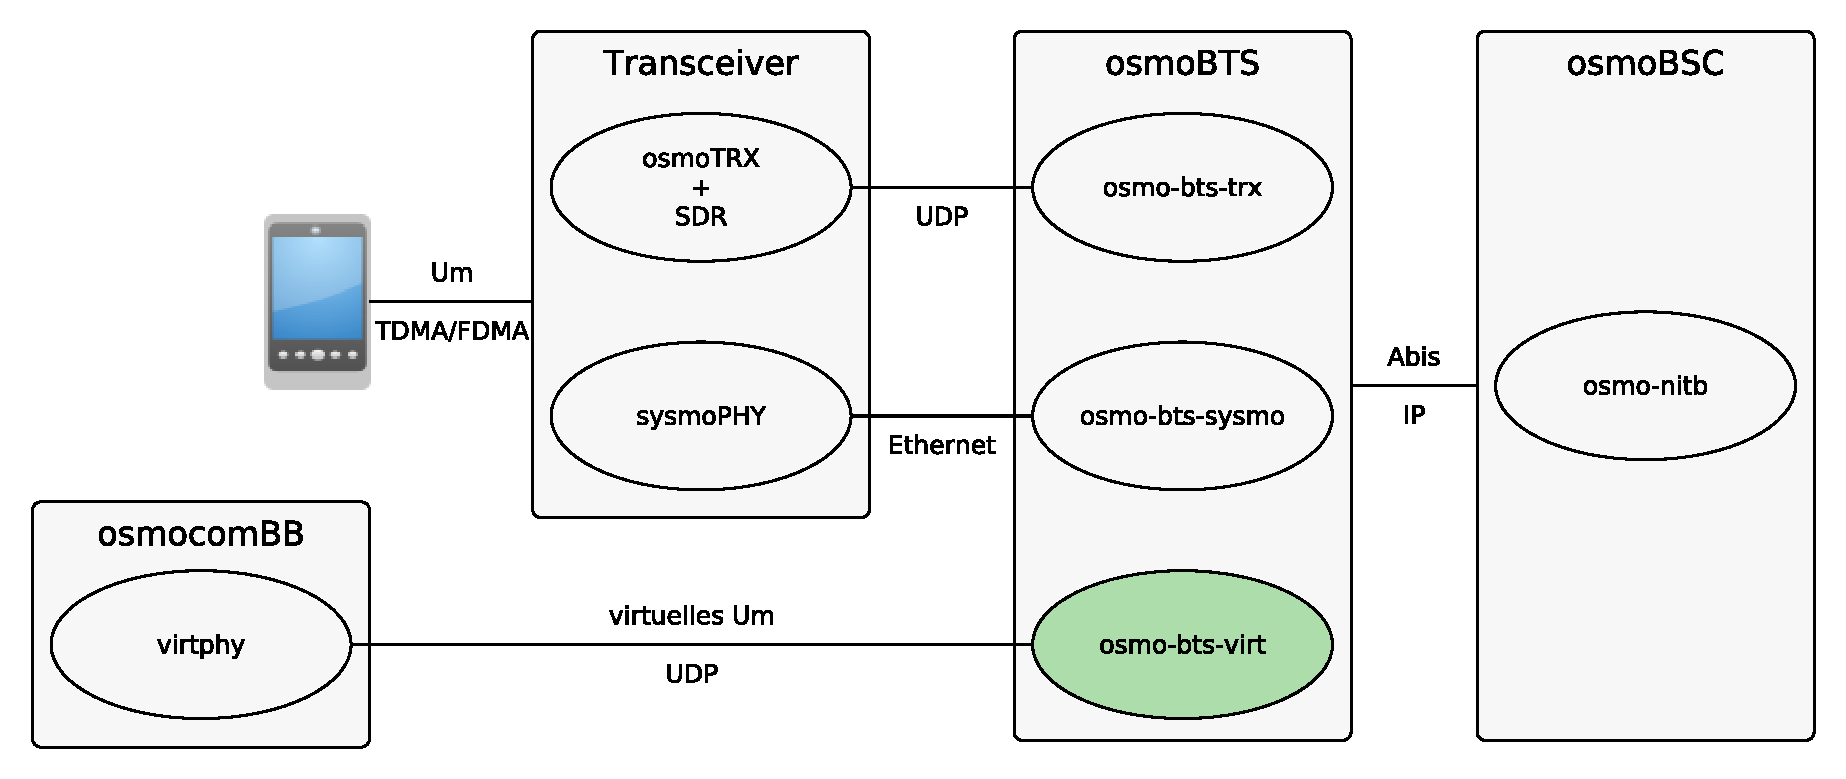
\includegraphics[width=1.0\linewidth]{figures/virt-bts-in-osmocom.pdf}
	\caption[Die Integration der virtuellen physikalischen Schicht in osmoBTS]{Die Integration der virtuellen physikalischen Schicht in osmoBTS, erstellt mit yEd} \label{fig:virt-bts-in-osmocom}
\end{figure}

Wie in obiger Grafik zu sehen, kann die virtuelle \ac{BTS} direkt über das virtuelle \ac{Um} mit verbundenen Mobiltelefonen kommunizieren und braucht keine Schnittstelle zu Transceiverhardware, wie \texttt{osmo-bts-trx} und \texttt{osmo-bts-sysmo}. Die Abis-Schnittstelle zum \ac{BSC} genauso wie die Protokollschichten 2 und 3 sind im \texttt{common} Teil des osmoBTS Projekts implementiert und werden aus diesem eingebunden. In der virtuellen Testumgebung wurde in dieser Arbeit \texttt{osmo-nitb} als \ac{BSC} verwendet (siehe \autoref{hdl:grundlagen_osmocom_OpenBSC}). Neben der Funktion als \ac{BSC} enthält \texttt{osmo-nitb} weitere Funktionalität von Komponenten des \ac{SS7} Netzwerks, wie zum Beispiel dem \ac{HLR}. Bei der Implementierung der physikalischen Schicht von \texttt{osmo-bts-virt} wurden folgende Aufgaben gelöst:
\begin{description}
\item[Build-Prozess] Das neue Programm wurde in den Automake Build-Prozess von osmoBTS eingebunden.
\item[Implementierung des \ac{SAP} der physikalischen Schicht zu höheren Schichten.] Die in \texttt{src/common} implementierten Protokolle \ac{LAPDm} und \ac{RR}, rufen verschiedene \ac{SAP}"=Rou\-tinen der physikalischen Schicht auf (siehe \autoref{hdl:sap}). Sie erwarten vom \ac{SAP} die korrekte Bestätigung (\ac{CON}-Primitives) ihrer Anfragen (\ac{REQ}-Primitives) und den Versand einiger \ac{IND}-Primitives von der physikalischen Schicht. Da andernfalls die höheren Schichten nicht korrekt arbeiten, wurde in der physikalischen Schicht die vollständige \ac{SAP}-Schnittstelle implementiert. Die Funktionalität der \ac{SAP}-Routinen wurde an das virtuelle \ac{Um} angepasst. Die Routine zur Übertragung einer Nutz- oder Signalisierungsnachricht verpackt diese zum Beispiel in \ac{GSMTAP} und schickt sie mit der \texttt{send()} Funktion von \texttt{virt\_um.c} an die konfigurierte Multicast-Adresse. Um die \ac{RR}-Schicht regelmäßig mit der aktuellen \ac{GSM}-Zeit zu versorgen, wurde ein alle 4.615 ms (Dauer eines Frames, siehe \autoref{hdl:a_tdma_fdma}) wiederkehrender Timerinterrupt definiert. Die Interrupt-Routine signalisiert der \ac{RR}-Schicht mit einem \ac{IND}-Primitive den Anfang eines neuen Frames. Die Funktionalität einiger \ac{SAP}-Routinen wird im virtuellen \ac{Um} nicht simuliert und wurde deshalb nicht implementiert. Dazu gehören zum Beispiel "`Frequency Hopping"', die Anpassung der Stärke des gesendeten Signals und die Verschlüsselung von \ac{RR}-Verbindungen.
\item[Parsen der eingehenden \ac{GSMTAP}-Nachrichten.] Da die Verwendung von \ac{GSMTAP} zur Nachrichtenübertragung innerhalb von Osmocom Programmen neu ist, fehlte die Logik zum Auslesen der Informationen des Headers. Diese wurde implementiert.
\item[Multiframe und \ac{TDMA}-Scheduling.] Damit ausgehende Nachrichten auf dem richtigen physikalischen und logischen Kanal gesendet werden, ist ein Scheduler notwendig. Es müssen periodische Aufgaben, wie das Broadcasting von \ac{SI}-Nachrichten und einmalige Aufgaben, wie der durch einen \ac{SAP}-Befehl initiierte Versand einer Nachricht, vom Scheduler für eine bestimmte \ac{FN} geplant und ausgeführt werden. In osmoBTS ist eine Kombination aus Multiframe- und \ac{TDMA}-Scheduler implementiert, dessen Basisfunktionalität im \texttt{common}-Teil zu finden ist. Die Funktionalität für die Planung von einmaligen und periodischen Aufgaben konnte übernommen werden. Die Routinen zur Ausführung, also in der Regel dem Versand einer Nachricht auf einem logischen Kanal, wurden neu geschrieben, so dass sie das virtuelle \ac{Um} für die Übertragung nutzen.
\item[Konfiguration der \ac{BTS} über \ac{VTY}.] Um die virtuelle \ac{BTS} über das Terminal konfigurieren zu können, wurde die \ac{VTY}-Schnittstelle implementiert. Die Konfiguration wird im physikalischen Modell der virtuellen \ac{BTS} (ein C-Struct) gespeichert und verschiedenen Routinen durch Shared-Memory zur Verfügung gestellt. Mit \ac{VTY} können zum Beispiel die Multicast-Adressen für Uplink und Downlink konfiguriert werden.
\item[Implementierung von \ac{OML}.] Beim Start meldet sich die \ac{BTS} bei ihrem zuständigen \ac{BSC} und nimmt anschließend auf der Abis Schnittstelle über den \ac{OML} mehrere Konfigurationen von diesem entgegen. So kann der \ac{BSC} zum Beispiel die Transceiverhardware der \ac{BTS} sowie aktive physikalische Kanäle und das zugewiesene Multiframe konfigurieren. Dabei handelt es sich um Konfigurationen auf physikalischer Ebene, die auf dem Hardwaremodell abgebildet werden müssen. Die \ac{OML}-Routinen wurden implementiert und auf dem physikalischen Modell der virtuellen \ac{BTS} abgebildet.
\end{description}

Zu Beginn der Arbeit war bereits die Implementierung eines Gerüsts für die virtuelle \ac{BTS} vorhanden. Das Gerüst umfasste die Einbindung und Konfiguration des Schedulers, die teilweise Implementierung der \ac{SAP} und \ac{OML}-Schnittstellen sowie Anpassungen an der \ac{VTY}-Schnittstelle der \ac{BTS}. Diese Implementierung wurde als Grundlage übernommen und erweitert. Sie befindet sich unverändert im Branch \texttt{laforge/virt-phy} des osmoBTS Github Repositories\footnote{\url{https://github.com/osmocom/osmo-bts.git}}. Die neue Implementierung, die mit ihrer Gegenseite im osmocomBB Projekt kompatibel ist, befindet sich im Branch \texttt{stumpf/virt"=phy}. Das Programm kann mit Automake und einem C-Compiler kompiliert und dann mit der ausführbaren Datei \texttt{osmo-bts-virtual} gestartet werden. Die Konfiguration erfolgt entweder über die \ac{VTY}-Konfigurationsschnittstelle, über die im osmoBTS Benutzerhandbuch nachgelesen werden kann, oder direkt über die Konfigurationsdatei im Projektordner. Beispielkonfigurationsdateien sind in \texttt{src/osmo-bts-virtual/example-configs} zu finden.

\section{OsmocomBB mit virtueller Um-Schnittstelle}

OsmocomBB ist eine Sammlung von Software rund um eine \ac{MS}, die in der Regel mit dem Konsolenprogramm Osmocon verwendet wird. Mit Osmocon ist es möglich, die Firmware im flüchtigen Speicher eines der unterstützten Mobiltelefone, wie zum Beispiel dem Motorola C123, auszutauschen. Über eine serielle Schnittstelle kann man das Telefon mit einem Linux Rechner verbinden und von diesem aus steuern, welches der vorkompilierten Firmware Pakete auf das Telefon geladen werden soll. Die einfachste Firmware dürfte \texttt{hello\_world} sein, die auf dem Display des Mobiltelefons einen Text ausgibt. \texttt{rssi\_scan} kann die \acp{RSSI}, also die Signalstärken der \ac{BTS} im Umkreis, messen und stellt diese auf dem Display dar. Die umfangreichste Firmware ist \texttt{layer1}. Sie implementiert die physikalische Schicht des \ac{GSM}-Protokollstapels für den Baseband-Prozessor. Für die Steuerung der Funktionen des Baseband-Prozessors und des \ac{DSP} von außen gibt es eine Kontrollschnittstelle. Diese Schnittstelle wird \ac{L1CTL} genannt und ist ein nicht spezifiziertes, osmocomBB-internes Protokoll. Osmocon bietet für den Zugriff auf die Schnittstelle ein lokales Linux-Domain-Socket an und leitet den Datenverkehr auf diesem über die serielle Schnittstelle zur \texttt{layer1}-Firmware weiter. Der Funktionsumfang des \ac{L1CTL}-Protokolls entspricht im Großen und Ganzen dem \ac{SAP} der physikalischen Schicht, die verschiedenen \ac{L1CTL}-Headertypen den \ac{SAP}-Primitives. Im Gegensatz zu einer internen \ac{SAP}-Schnittstelle ist die externe \ac{L1CTL}-Schnittstelle aber von außen über das Socket zugänglich. Mehrere sogenannte L23-Apps, die die Funktionalität der höheren \ac{GSM}-Protokollschichten implementieren, nutzen \ac{L1CTL} für die Steuerung der physikalischen Schicht des verbundenen Mobiltelefons. Die L23-App \texttt{ccch\_scan} ist ein passiver \ac{CCCH} und \ac{BCCH} Sniffer, der empfangene Nachrichten über \ac{GSMTAP} protokolliert. \texttt{cell\_log} macht einen vollständigen Messdurchlauf der Empfangsstärken aller \ac{ARFCN} und gibt das Ergebnis auf der Kommandozeile aus. Besonders interessant ist die L23-App \texttt{mobile}, die die Funktionalität eines klassischen Mobiltelefons simuliert und über eine \ac{VTY}-Schnittstelle gesteuert werden kann. Damit kann der Nutzer zum Beispiel eine Telefonnummer anrufen, eine \ac{SMS} versenden oder nach \ac{BTS} in Reichweite suchen. 

Die Struktur des Projekts trennt strikt zwischen Host-Software und Target-Software. Im Ordner \texttt{src/host} befinden sich alle Anwendungen, die auf dem Linux-Rechner laufen, wie die L23-Apps und Osmocon. In \texttt{src/target} wird die Software für das Mobiltelefon gesammelt. Sie muss zuerst cross-kompiliert und dann mit Osmocon geladen werden. Das sind alle Firmware- Implementierungen wie \texttt{layer1} oder \texttt{rssi\_scan}. Da die Anwendung für das virtuelle \ac{MS} nicht auf dem Mobiltelefon, sondern auf dem Rechner ausgeführt wird, wurde der Ordner \texttt{virt\_phy} für dessen Entwicklung in \texttt{src/host} angelegt. Folgende Grafik zeigt die Schnittstellen der virtuellen physikalischen Schicht (\texttt{virthphy}) in osmocomBB im Vergleich mit anderen Target- und Host-Anwendungen.

\begin{figure}[H]
	\centering 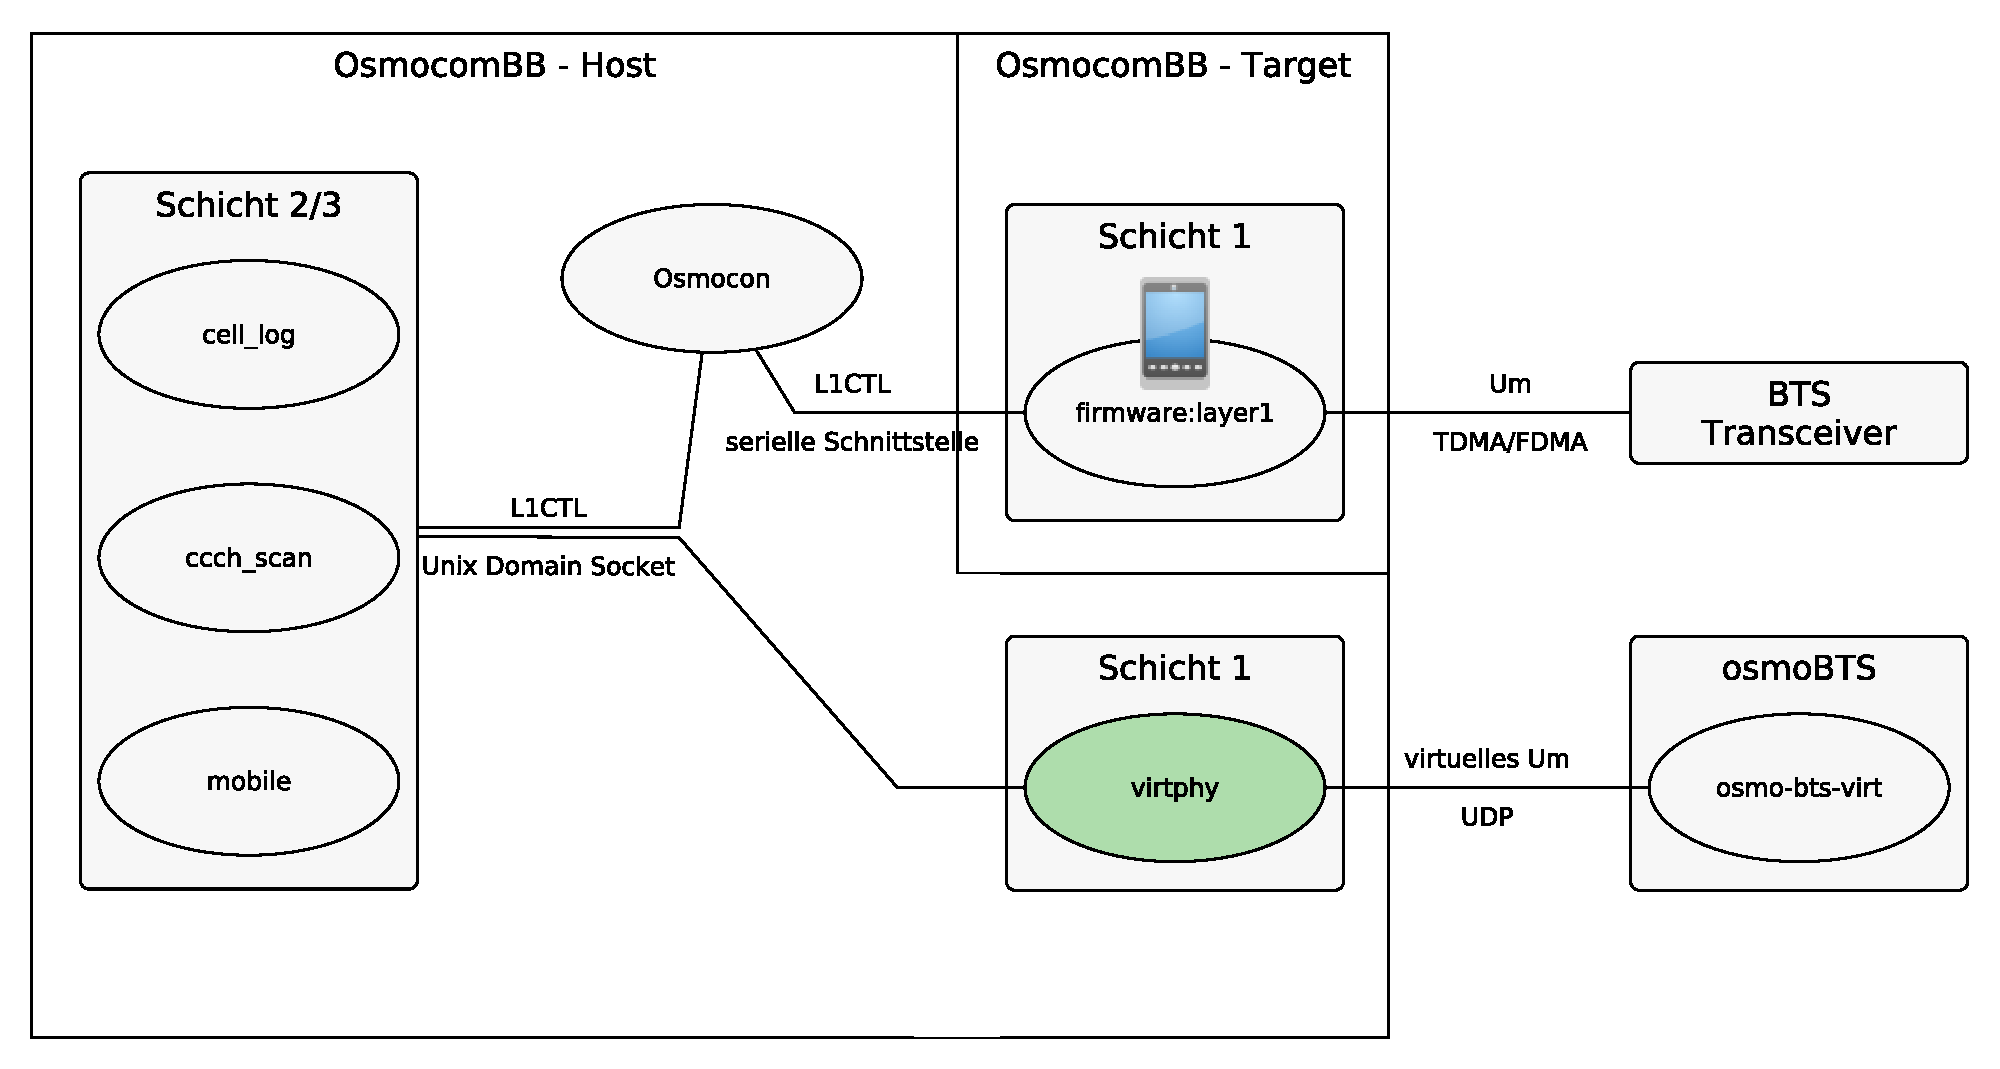
\includegraphics[width=1.0\linewidth]{figures/virt-bb-in-osmocom.pdf}
	\caption[Die Integration der virtuellen physikalischen Schicht in osmocomBB]{Die Integration der virtuellen physikalischen Schicht in osmocomBB, erstellt mit yEd} \label{fig:virt-bb-in-osmocom}
\end{figure}

In \autoref{fig:virt-bb-in-osmocom} kann man erkennen, dass \texttt{virtphy} die strikte Trennung der physikalischen Schicht von den höheren Schichten einhält. \texttt{virtphy} implementiert nur die physikalische Schicht der virtuellen \ac{MS}, die höheren Protokollschichten liegen in den L23-Apps. Die Osmocon Anwendung wurde nicht mit eingebunden, da dessen Hauptfunktionalität, Firmware auf ein Target zu laden, nicht benötigt wird. Neben der Schnittstelle zum virtuellen \ac{Um}, bietet die virtuelle physikalische Schicht also auch die \ac{L1CTL}-Schnittstelle über ein Linux-Domain-Socket an. Der Funktionsumfang von \texttt{virtphy}, das als eigener Prozess auf dem Rechner läuft, entspricht in etwa der \texttt{layer1}-Firmware. Alle Aufgaben die bei der Implementierung der gelöst wurden sind im Folgenden zusammengefasst.
\begin{description}
\item[Build-Prozess.] Die \texttt{virt-phy} Anwendung wurde in den Build-Prozess von osmocomBB eingebunden. Wie in osmoBTS wird Automake verwendet.
\item[Implementierung des \ac{L1CTL}-Sockets] Die Funktionalität zur Erstellung und Konfiguration des \ac{L1CTL}-Sockets wurde aus Osmocon übernommen und in einer eigenen Datei \texttt{l1ctl\_sock} gekapselt.
\item[Parsen von \ac{GSMTAP}.] Die \ac{GSMTAP}-Logik wurde über geteilte Ressourcen aus der virtuellen \ac{BTS} Implementierung eingebunden. 
\item[Implementierung der \ac{L1CTL}-Schnittstelle.] Um das \ac{L1CTL}-Protokoll implementieren zu können wurde die Kommunikation zwischen der \texttt{layer1}-Firmware und verschiedenen L23-Apps analysiert. Von der L1CTL-Schnittstelle gibt es keine offizielle Dokumentation. Die Aufgaben der verschiedenen \ac{L1CTL}-Routinen wurden durch Debugging und Codeanalyse, sowie teilweise Dokumentation im Code herausgefunden, was deren Implementierung in der virtuellen physikalischen Schicht ermöglichte. Das \ac{L1CTL}-Protokoll orientiert sich dabei stark am \ac{SAP} der physikalischen Schicht und definiert verschiedene \ac{REQ}, \ac{IND} und \ac{CON}-Nachrichtentypen (siehe \autoref{hdl:sap}). Um Fehler in den L23-Apps zu vermeiden, wurde die Schnittstelle vollständig implementiert und die ausgeführten \ac{L1CTL}-Routinen an das virtuelle \ac{Um} angepasst. Unter anderem wurde die Funktionalität der Routinen zur Messungen von Signalstärken, Senden einer Signalisierungsnachricht, dem Wechsel in den dedizierten Modus und der Synchronisation mit einer \ac{BTS} implementiert. Alle Nachrichten des \ac{L1CTL}-Protokolls sind mit einer kurzen Beschreibung und dem Status der zugehörigen Routine in der Implementierung der virtuellen physikalischen Schicht, in \autoref{hdl:a_l1ctl-routines} hinterlegt.
\item[Routine zur Messung von Signalstärken.] Auf dem virtuellen \ac{Um} gibt es keine unterschiedlichen Signalstärken. Alle Nachrichten auf dem Multicast-Socket werden mit gleicher Qualität empfangen. Da die \ac{MS} sich jedoch immer mit der \ac{BTS} mit dem besten Empfang verbindet, ist die Simulation der Signalstärken wichtig. Durch die Konfiguration unterschiedlicher Signalstärken für verschiedene \acp{BTS}, kann Einfluss darauf genommen werden, mit welcher \ac{BTS} sich das \ac{MS} verbindet. Die Messung von Signalstärken wird über die \ac{L1CTL}-Nachricht \texttt{L1CTL\_PM\_REQ} von der L23-App, für eine Liste von \acp{ARFCN}, gestartet. Die in der Antwort \texttt{L1CTL\_PM\_CON} zurückgegebenen Messwerte der virtuellen physikalischen Schicht wurden so definiert: \acp{ARFCN} von denen regelmäßig eine Nachricht auf dem virtuellen \ac{Um} empfangen wird, erhalten die maximale Signalstärke (> -63 dBm in \ac{GSM}), alle anderen die minimale Signalstärke (< -110 dBm in \ac{GSM}). Damit wird gewährleistet, dass die \ac{RR}-Schicht nur die Verbindung mit verfügbaren \ac{ARFCN} initiiert. Des Weiteren kann mit Kommandozeilenparametern von \texttt{virtphy}, für jede \ac{ARFCN} ein Signalstärkereduktionswert angegeben werden, um den der zurückgegebene Signalstärkemesswert dieser \ac{ARFCN} reduziert wird. Damit kann der Anwender unterschiedlichen Empfang für die \ac{BTS} auf dem virtuellen \ac{Um} konfigurieren und so beeinflussen, mit welcher \ac{BTS} sich das \ac{MS} verbindet.
\item[Routine zur Synchronisation der \ac{MS} mit einer \ac{BTS}.] Die \ac{RR}-Schicht in der L23-App schickt die \ac{L1CTL}-Nachricht \texttt{L1CTL\_FBSB\_REQ}, um sich mit einer ausgewählten \ac{ARFCN} zu verbinden, sobald ihr die Signalstärkemesswerte aller \acp{ARFCN} vorliegen. Im Gegensatz zur realen Funkschnittstelle ist auf dem virtuellen \ac{Um} keine Frequenzsynchronisation nötig, da auf dem Multicast-Socket die Nachrichten aller \ac{BTS} empfangen werden. Auf dem virtuellen \ac{Um} senden die \acp{BTS} außerdem keine Nachrichten auf dem \ac{SCH}, der für die zeitliche Synchronisation mit dem Multiframe verwendet wird. Die Synchronisationsmechanismen wurden deshalb wie folgt an das virtuelle \ac{Um} angepasst. Die Synchronisation mit einer \ac{ARFCN} wird durch das Herausfiltern aller Nachrichten von anderen \acp{ARFCN} erreicht. Die zeitliche Synchronisation ist auf der realen Funkschnittstelle nötig, um die empfangenen Nachrichten den korrekten logischen und physikalischen Kanälen zuordnen zu können. Auf dem virtuellen \ac{Um} sind die Informationen, die für die Zuordnung benötigt werden (\ac{FN} und \ac{TDMA}-Zeitschlitz), im \ac{GSMTAP}-Header jeder Nachricht verfügbar. Insofern wird die zeitliche Synchronisation dafür nicht benötigt. Der Scheduler muss für die Planung von Aufgaben für eine \ac{FN} in der Zukunft aber die aktuelle \ac{FN} kennen. Um dem Scheduler diese Information zu Verfügung zu stellen, aktualisiert die virtuelle physikalische Schicht, mit jeder eingehenden Nachricht von der synchronisierten \ac{BTS}, eine lokale \ac{FN} im Modell der virtuellen \ac{MS}. Diese wird dem Scheduler zur Verfügung gestellt.
\item[Scheduling.] Die Implementierung des Schedulers besteht aus der Planungslogik, die Aufgaben für den richtigen physikalischen und logischen Kanal einplant und der Ausführungslogik der Aufgaben. Der Scheduler wird, sobald die \ac{MS} mit einer \ac{BTS} verbunden ist, bei jeder auf dem virtuellen \ac{Um} empfangenen Nachricht ausgeführt. Der Scheduler ist damit nicht aktiv zeitgesteuert, sondern passiv und abhängig von eingehenden Nachrichten. Da das \ac{MS} von der \ac{BTS} jedoch regelmäßig Nachrichten auf dem \ac{BCCH} und anderen Kanälen erhält, ist diese einfache und passive Lösung ausreichend. Der Scheduler wird mit dieser Lösung nicht für jede \ac{FN} aufgerufen und führt deshalb der Reihe nach alle Aufgaben aus, die für die aktuelle und kleinere \ac{FN} geplant wurden. Für den Scheduler wurde bewusst eine einfache Variante gewählt. In den aufgezeichneten Mitschnitten konnte die Lösung die richtige Reihenfolge und \ac{FN} der gesendeten Nachrichten gewährleisten und war somit ausreichend.
\item[Schnittstelle zum \ac{SIM}.] Für die Ausführung der Sicherheitsalgorithmen benötigt die \ac{MS} eine Schnittstelle zum \ac{SIM}. In der \texttt{layer1}-Firmware ist diese implementiert und wird über eine \ac{L1CTL}-Routine für höhere Schichten zur Verfügung gestellt. Auch das virtuelle \ac{MS} braucht Zugriff auf Daten und Sicherheitsalgorithmen der \ac{SIM}-Karte. Dazu kann entweder das \ac{SIM} simuliert, oder die Schnittstelle zu einem \ac{SIM}-Kartenlesegerät implementiert werden. In der L23-App \texttt{mobile} kann eine \texttt{test-sim} Option aktiviert werden, mit der sie eine \ac{SIM}-Karte simuliert und zur Verfügung stellt. Die \ac{L1CTL}-Routine für den Zugriff auf die \ac{SIM}-Karte wurde deshalb nicht implementiert, sondern stattdessen die Aktivierung der \texttt{test-sim} Option vorausgesetzt. Damit ein virtuelles \ac{MS} Zugriff auf alle Netzwerkdienste hat, muss die \ac{SIM}-Karte einen gültigen Netzteilnehmer identifizieren. Dazu muss die auf der Test-\ac{SIM} gespeicherte \ac{IMSI} auch im \ac{HLR} vorhanden sein. In osmoNITB ist das \ac{HLR} durch eine SQLite-Datenbank realisiert, in die die Werte der Netzteilnehmer eingetragen werden.
\end{description}

Einige Funktionen der \ac{Um}-Schnittstelle werden aktuell (Stand Mai 2017) noch nicht von den Implementierungen für das virtuelle \ac{MS} und \ac{BTS} unterstützt. Dazu gehören Frequency Hopping, Sprachdatenübertragung, sowie Kodierung und Verschlüsselung des Nachrichtenverkehrs. Für die praktische Durchführung des \ac{MitM}-Angriffs war die Implementierung dieser Funktionen nicht notwendig. Für die virtuelle physikalische Schicht gibt es zudem keine \ac{VTY} Konfigurationsschnittstelle. Die Konfiguration erfolgt über Kommandozeilenparameter beim Start des Programms.

\section{Die Validierung der Manipulation der Setup-Nachricht mit Testdaten}\label{hdl:coder-impl}

Wegen der fehlenden Kanalkodierung und Verschlüsselung auf dem virtuellen \ac{Um} wurden das Kommandozeilenprogramm \texttt{dummycoder} und das Python Skript \texttt{xor\_hexstrings} geschrieben. Beide Programme befinden sich im osmoMITM\footnote{\url{https://github.com/BastusIII/osmo-mitm.git}} Repository.

Die Kodierungsfunktionalität wurde in \texttt{coder.c} implementiert. Für die Kodierung und Dekodierung einer Nachricht auf dem  \ac{FACCH} wurden die Funktionen \texttt{facch\_encode()} und \texttt{facch\_decode()} geschrieben, für alle anderen Signalisierungskanäle \texttt{xcch\_encode()} und \texttt{xcch\_decode()}. Die Funktionen nehmen als Eingangsdaten das beliebige Ergebnis eines Zwischenschrittes der Kanalkodierung entgegen und geben die Zwischenergebnisse aller angewendeten Kodierungsfunktionen zurück. Der Grund für die Trennung von \ac{FACCH} von anderen Signalisierungskanälen liegt in den unterschiedlichen kombinierten Kodierungsverfahren (siehe \autoref{hdl:encoding}). Die Kodierungsverfahren für Firecode und Faltungskodierung werden von der libosmocore Bibliothek zur Verfügung gestellt und wurden aus dieser verwendet. Die Logik für Interleaving und Burstmapping wird nicht von der Bibliothek angeboten, konnte aber aus \texttt{osmo-bts-trx} übernommen werden.

Das Programm \texttt{dummycoder} liest Hexstrings aus Textdateien ein, kodiert oder dekodiert sie auf Wunsch des Anwenders und speichert das Ergebnis wieder ab. Dafür verwendet es die von \texttt{coder.c} bereitgestellten Funktionen und enthält selbst nur die Logik zum Einlesen und Formatieren der Eingangs- und Ergebnisdaten. Das Python Skript \texttt{xor\_hexstrings} ließt zwei Hexstrings ein und verknüpft diese mit der \ac{XOR}-Operation. Dadurch lässt sich die Stromverschlüsselung einer \ac{GSM}-Nachricht simulieren.

Im Ordner \texttt{tests} befinden sich zwei Testfälle, in denen die beiden Programme verwendet werden, um eine Beispiel Setup-Nachricht zu kodieren und zu manipulieren. Die Ergebnisse aus \texttt{tests/encode\_decode\_test} sind in die Beispieldaten der Kanalkodierung in \autoref{hdl:encoding} eingeflossen. Das Skript in \texttt{tests/setup\_manip\_test} wurde verwendet, um die Manipulation der Telefonnummer in einer Setup-Nachricht anhand von Beispieldaten zu validieren. Die Konsolenausgabe des Tests ist in \autoref{hdl:a_example_setup_manip} zu finden.

\section{Die Validierung des Angriffs mit einem Man-in-the-Middle im virtuellen Um}\label{hdl:mitm_impl}

Für die praktische Nachstellung des in \autoref{hdl:theroetical-attack} ausgearbeiteten Angriffs wurde ein \ac{MitM} auf dem virtuellen \ac{Um} implementiert. Der \ac{MitM} hat Zugriff auf den Uplink und Downlink des virtuellen und eines korrumpierten \ac{Um} und stellt die Verbindung zwischen beiden her. Alle \ac{MS} die sich mit dem korrumpierten virtuellen \ac{Um} verbinden, kommunizieren so über den \ac{MitM} mit dem Netzwerk und der \ac{MitM} hat Zugriff auf den kompletten Datenverkehr. Die Implementierung besteht aus einem Rahmen, der die Funktionalität der zwei virtuellen \ac{Um}-Schnittstellen anbietet, und einer Verarbeitungslogik. Die Verarbeitungslogik wird über zwei als extern deklarierte Callbackfunktionen eingebunden. Der Uplink-Callback wird bei einer eingehenden Nachricht auf dem korrumpierten Uplink aufgerufen, sein Rückgabewert an das \ac{Um} weitergeleitet. Der Downlink-Callback wird bei einer eingehenden Nachricht auf dem Downlink aufgerufen, sein Rückgabewert an das korrumpierte \ac{Um} weitergeleitet. Ein Rückgabewert von NULL bedeutet, dass die Nachricht blockiert wurde. Damit können Nachrichten von der Verarbeitungslogik verändert, verzögert oder abgefangen werden. \autoref{fig:virtual-um-mitm} zeigt, wie die \ac{MitM}-Verarbeitungsroutinen im \ac{MitM}-Gerüst eingebunden sind und die Vermittlung von Nachrichten zwischen virtuellen \ac{Um} und korrumpiertem virtuellen \ac{Um}.

\begin{figure}[H]
	\centering 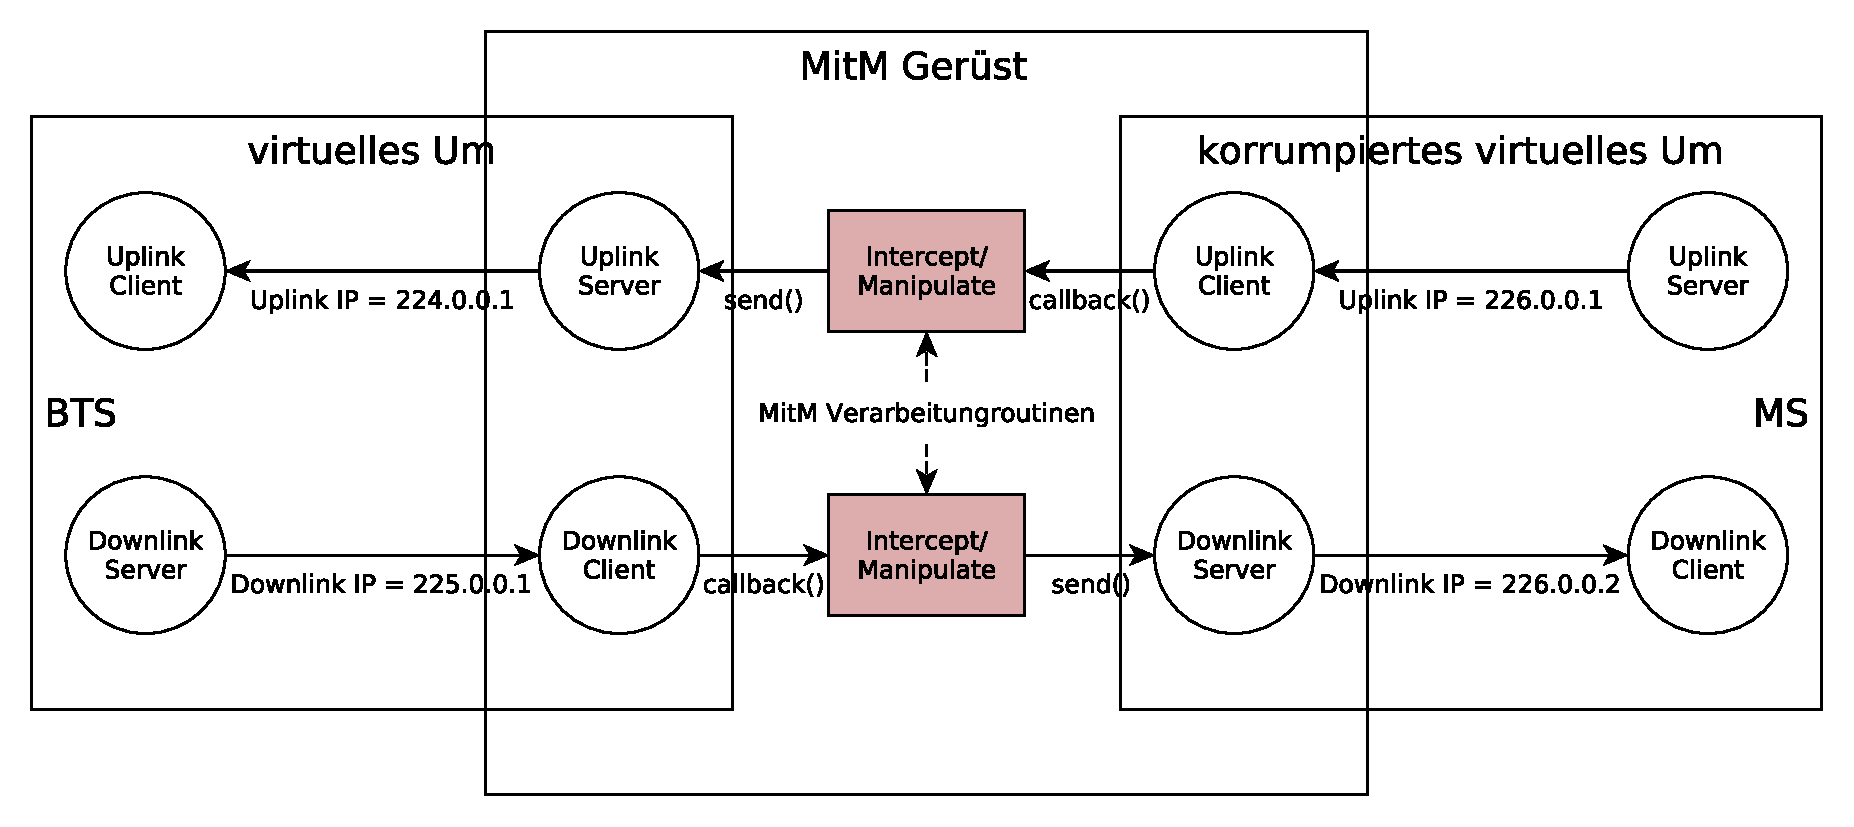
\includegraphics[width=1.0\textwidth]{figures/mitm_in_virt_um_with_multicast.pdf}
	\caption[Die MitM-Implementierung im virtuellen Um]{Die \ac{MitM}-Implementierung im virtuellen \ac{Um}, erstellt mit yEd} \label{fig:virtual-um-mitm}
\end{figure}

Das \ac{MitM}-Gerüst muss über Kommandozeilenparameter mit den \ac{IP}-Adressen von Uplink und Downlink des \ac{Um} und des korrumpierten \ac{Um} konfiguriert werden, da es die Logik für den Aufbau der virtuellen \ac{Um}-Schnittstellen enthält. Von den Verarbeitungsroutinen benötigte, zusätzliche Optionen können über einen Optionshandler definiert werden. Eine Verarbeitungsroutine muss neben dem Optionshandler nur die beiden Funktionen implementieren die empfangene Nachrichten analysieren und bearbeiten. Sie kann deshalb leicht ausgetauscht werden. Im Zuge der Masterarbeit wurden drei Verarbeitungslogiken entwickelt. \texttt{SimpleForward} leitet alle Nachrichten, ohne sie zu verändern, sobald sie eingehen, sofort weiter. \texttt{ImsiCatcher} realisiert einen \ac{IMSI}-Catcher, der eine \ac{GSM} Schwachstelle ausnutzt, um die aktuellen \acp{TMSI} der Netzteilnehmer ihren \acp{IMSI} zuzuordnen und damit ihre Identität offenlegt. \texttt{CallSetupManipulation} kombiniert die Funktionalität des \ac{IMSI}-Catchers mit der im Zuge der Masterarbeit ausgearbeiteten Identifikation und Manipulation der Setup-Nachricht (siehe \autoref{hdl:theroetical-attack}), um ein ausgehendes Telefonat umzuleiten. Die einfachste Routine ist in folgendem Codebeispiel zu sehen. Das C-Struct \texttt{msgb} wird innerhalb von Osmocom verwendet, um eine Nachricht mit Nutzdaten und mehreren Headern zu definieren.\\

%\begin{adjustbox}{max width={0.95\textwidth}, padding=20pt 10pt 10pt 10pt, frame, center}
\begin{lstlisting}[caption={[Die Simple-Forward Verarbeitungsroutine des MitM]Die Simple-Forward Verarbeitungsroutine des \ac{MitM}}, label={lst:simple_forward}, boxpos=c, frame=single, style=CStyle, numbers=none]
#include <osmocom/core/msgb.h>

/**
 * Simple Forward hat keine zusätzlichen Optionen.
 */
void handle_suboptions(int argc, char **argv)
{
	return;
}
/**
 * Rückgabe und damit einfache Weiterleitung der originalen Nachricht.
 */
struct msgb* downlink_rcv_cb_handler(struct msgb *msg) {
	return msg;
}
/**
 * Rückgabe und damit einfache Weiterleitung der originalen Nachricht.
 */
struct msgb* uplink_rcv_cb_handler(struct msgb *msg) {
	return msg;
}
\end{lstlisting}
%\end{adjustbox}

Die Implementierung des \ac{MitM} Frameworks auf dem virtuellen \ac{Um} mitsamt den Verarbeitungsroutinen ist im osmoMITM\footnote{\url{https://github.com/BastusIII/osmo-mitm.git}} Repository hinterlegt.

\subsection{Die Verarbeitungsroutine des IMSI-Catchers}

Die Identitäten auf dem \ac{Um} werden durch die Verwendung einer temporären ID, der \ac{TMSI}, verschleiert. Der Angreifer im vorgestellten \ac{MitM}-Angriff möchte nur die ausgehenden Anrufe von einem bestimmten Netzteilnehmer umleiten. Damit dieser eindeutig vom Angreifer identifiziert werden kann, wird die aktuelle \ac{TMSI} benötigt, die ihm vom Netzwerk zugewiesen wurde. Da die Zuweisung der \ac{TMSI} im "`Location Updating Accept"' oder "`TMSI Reallocation Command"' verschlüsselt geschieht, kann sie nicht aus dem Datenverkehr auf dem \ac{Um} ausgelesen werden. Ein sogenannter \ac{IMSI}-Catcher nutzt Schwachstellen im \ac{GSM}-Standard aus, um die Identitäten verbundener Netzteilnehmer zu sammeln. Da der Angriff die Kenntnis der Identität des Opfers voraussetzt, wurde das \ac{MitM}-Gerüst im virtuellen \ac{Um} um die Logik eines \ac{IMSI}-Catchers erweitert.

Die Grundlage des \ac{IMSI}-Catchers ist eine falsche \ac{BTS}, die auf alle eingehenden Anfragen von verbundenen \ac{MS} mit einem "`Identity Request"' die \ac{IMSI} des \ac{MS} abfragt, diese sammelt und einem Angreifer zur Verfügung stellt. Der \ac{GSM}-Standard spezifiziert, dass eine \ac{MS} während einer \ac{RR}-Verbindung eingehende Identity-Requests immer erwarten und beantworten muss \citepauthor[Kap. 4.3.3.2]{3gpp:24.008}. Da der Identity-Request des Angreifers erfolgt, bevor die Verschlüsselung aktiviert wird, muss er sich darum nicht kümmern.

Hat ein Angreifer Zugriff auf den Datenverkehr auf dem \ac{Um} gibt es zudem mehrere Möglichkeiten, den IMSI-Catcher so zu erweitern, dass er die temporäre Identität (\ac{TMSI}) von Netzteilnehmern auf dem \ac{Um} ihrer eindeutigen Identität (\ac{IMSI}, \ac{MSISDN}) zuordnen kann. Überwacht der Angreifer mit einem passiven Sniffer den \ac{PCH} einer \ac{BTS}, kann er die von einer sogenannten "`Silent \ac{SMS}"' an die \ac{MSISDN} des Opfers ausgelösten Paging Nachrichten analysieren. In einer Paging Nachricht steht in der Regel die \ac{TMSI} des Opfers \citepauthor[Kap. 3.3.2.1.1]{3gpp:04.18}, die der Angreifer so dessen \ac{MSISDN} zuordnen kann. Dem Opfer wird der Empfang einer Silent \ac{SMS} nicht angezeigt, er hat also keine Möglichkeit, den Angriff zu bemerken.

Der in dieser Arbeit implementierte \ac{IMSI}-Catcher setzt einen aktiven Eingriff in den Datenverkehr auf dem \ac{Um} voraus. Der von der \ac{IMSI}-Catcher Verarbeitungsroutine manipulierte Nachrichtenfluss ist in \autoref{fig:mitm-imsi-catcher} dargestellt.

\begin{figure}[H]
	\centering \includegraphics[width=1.0\linewidth]{figures/mscgen/gsm_imsi_catcher.pdf}
	\caption[Die IMSI-Catcher Verarbeitungsroutine des MitM]{Die \ac{IMSI}-Catcher Verarbeitungsroutine des \ac{MitM}, verifiziert mit Wireshark-Mitschnitt auf virtuellem \ac{Um}, siehe \autoref{lst:mitm_attack_wireshark}} \label{fig:mitm-imsi-catcher}
\end{figure}

Die Identität des \ac{MS} wird in der \ac{SABM}-Anfrage (siehe \autoref{fig:mitm-imsi-catcher}, Teil 1) an das Netzwerk entweder als \ac{IMSI} oder als \ac{TMSI} angehängt. Ist die angehängte \ac{TMSI} in einer Anfrage unbekannt, so wird die Nachricht vom Angreifer mit einem Identity-Request beantwortet, der die zugehörige \ac{IMSI} vom \ac{MS} abfragt. Die Identity Response mit der \ac{IMSI} vom \ac{MS} wird abgefangen und die Zuordnung der \ac{IMSI} zur \ac{TMSI} in einer Datenstruktur abgespeichert (siehe Teil 2). Anschließend wird die \ac{RR}-Verbindung mit einem Channel Release vom \ac{MitM} beendet (siehe Teil 3). Das \ac{MS} sendet und empfängt nach dem \ac{DISC} keine weiteren Nachrichten mehr auf dieser Verbindung. Da das Netzwerk vom Release nichts mitbekommt, horcht es noch eine Weile auf der \ac{RR}-Verbindung, wird aber, nachdem es eine bestimmte Zeit keine Nachrichten vom \ac{MS} erhalten hat, von einem Fehler ausgehen und die Verbindung ebenfalls beenden. Da die blockierten Anfragen, wie der Location Update-Request, in der Regel automatisch vom \ac{MS} generiert werden, bemerkt der Nutzer den Angriff nicht.

Der \ac{IMSI}-Catcher auf dem virtuellen \ac{Um} ist wie ein Zustandsautomat aufgebaut. Jeder Nachricht, die als nächstes erwartet wird, wurde ein Zustand zugewiesen. Die beim Zustandsübergang ausgeführten Funktionen definieren, ob und wie die eingegangene Nachricht verändert wird. Mit dem \ac{IMSI}-Catcher wurden Wireshark Mitschnitte mit erfolgreichen Zuordnungen von \ac{TMSI} zu \ac{IMSI} auf dem virtuellen \ac{Um} erstellt (siehe \autoref{lst:mitm_attack_wireshark}). 

\subsection{Die Verarbeitungsroutine der Setup Manipulation}
Die in \autoref{hdl:theroetical-attack} beschriebe Logik für die Manipulation der kodierten und verschlüsselten Setup-Nachricht wurde in dieser Verarbeitungsroutine für den \ac{MitM} auf dem virtuellen \ac{Um} implementiert. Das Ziel ist die Umleitung des Anrufs, indem die angerufene Telefonnummer ausgetauscht wird.

Die Funktionalität der Implementierung umfasst die Identifikation des Opfers, wofür die Logik der oben beschriebenen \ac{IMSI}-Catcher Verarbeitungsroutine eingebunden wurde. Des Weiteren wird die Datenübertragung auf vom identifizierten Opfer ausgehende Anrufe analysiert. Wie die dafür zuständige Setup-Nachricht im Nachrichtenfluss erkannt werden kann, wurde in \autoref{hdl:call-setup-message-flow-analysis} herausgearbeitet. Als Letztes ist die Manipulation der Setup-Nachricht implementiert. Die dafür zuständige Funktion erwartet die \ac{LAPDm}-Nachricht verschlüsselt und kanalkodiert, wofür die Funktionalität des Coders eingebunden wurde (siehe \autoref{hdl:coder-impl}). Das Programm wird über Kommandozeilenparameter mit den als bekannt vorausgesetzten Werten initialisiert und erwartet beim Start deshalb die Telefonnummer des angerufenen Opfers (\texttt{msisdn-called}), die \ac{IMSI} des anrufenden Opfers (\texttt{imsi-victim}) und das Offset der Telefonnummer in der Call Setup-Nachricht (\texttt{msisdn-to-setup-offset}). In folgendem Codebeispiel kann man erkennen, dass die Funktion \texttt{manip\_setup\_msg()}, in der die Manipulation der Setup-Nachricht stattfindet, mit kodierten Daten aufgerufen wird. Die Kodierung übernimmt die \texttt{xcch\_encode()} Funktion aus dem Coder. Die Daten werden nicht verschlüsselt, was ein zusätzliches \ac{XOR} mit einem Schlüsselstrom wäre. Der Nachweis, dass der Angriff mit verschlüsselten Daten funktioniert, ist hier nicht mehr nötig. Er wurde in den Tests in \autoref{hdl:coder-impl} erbracht.\\

%\begin{adjustbox}{max width={0.95\textwidth}, padding=20pt 10pt 10pt 10pt, frame, center}
\begin{lstlisting}[caption={[Die Callbackfunktion für eingehende Nachrichten auf dem Uplink, Auszug aus der Setup-Manipulation Verarbeitungsroutine des MitM]Die Callbackfunktion für eingehende Nachrichten auf dem Uplink, Auszug aus der Setup-Manipulation Verarbeitungsroutine des \ac{MitM}}, label={lst:setup_manip1}, boxpos=c, frame=single, style=CStyle, numbers=none]
// Auszug aus dem Uplink Callback der Setup Manipulation MitM Verarbeitungsroutine.
// msg enthält die empfangene Originalnachricht.
struct msgb* uplink_rcv_cb_handler(struct msgb *msg)
{
	// Extraktion des GSMTAP Headers aus der Nachricht
	struct gsmtap_hdr *gh = msgb_l1(msg);
	// Puffer für manipulierte Nachricht
	struct msgb *manip_msg;
	// Puffer für kodierte Originalnachricht. LEN_BURSTMAP_XCCH ist 4*116.
	uint8_t encoded_msg[LEN_BURSTMAP_XCCH / 8];
	// Puffer für kodierte, manipulierte Nachricht
	uint8_t encoded_manip_msg[LEN_BURSTMAP_XCCH / 8];
	(...)
	switch(mitm_state) {
	(...)
	case STATE_IMSI_CATCHER_SABM:
		// Kopieren des GSMTAP Headers (l1h) in den Puffer für die manipulierte Setup 
		// Nachricht
		manip_msg->l1h = msgb_put(manip_msg, sizeof(*gh));
		memcpy(manip_msg->l1h, gh, sizeof(*gh));
		(...)
		manip_msg->l1h = msgb_put(manip_msg, sizeof(*gh));
		// Kanalkodierung der Nachricht. Der Kodierungsfunktion aus coder.c wird mit
		// der unkodierten Nachricht vom Typ PLAIN aufgerufen. Das wird Ergebnis im  
		// Puffer encoded_msg abgespeichert.
		xcch_encode(PLAIN, msgb_data(msg), encoded_msg, NULL, NULL, NULL);
		// Die Funktion die die Telefonnummer in der Setup-Nachricht austauscht. 
		// Die manipulierte Nachricht wird im Puffer encoded_manip_msg abgespeichert
		manip_setup_msg(encoded_manip_msg, encoded_msg, LEN_BURSTMAP_XCCH / 8);
		// Dekodieren der manipulierten Setup-Nachricht. Das Ergebnis wird im msgb 
		// Puffer manip_msg an Position des LAPDm Header abgespeichert (l2h).
		xcch_decode(BURSTMAP_XCCH, encoded_manip_msg, NULL, NULL, NULL, manip_msg->l2h);
		(...)
		break;
	}
	(...)
	// Der Rückgabewert der Verarbeitungsroutine ist die manipulierte Nachricht, 
	// vom MitM Gerüst wird diese also an die BTS weitergeleitet
	return manip_msg;
}
\end{lstlisting}
%\end{adjustbox}

Mit dem \ac{MitM} und der Setup Manipulation Verarbeitungslogik konnte der Angriff erfolgreich auf dem virtuellen \ac{Um} ausgeführt und damit seine Machbarkeit gezeigt werden. Der Wireshark Mitschnitt des Nachrichtenverkehrs auf dem virtuellen \ac{Um} ist im Anhang in \autoref{lst:mitm_attack_wireshark} zu finden.